% This example An LaTeX document showing how to use the l3proj class to
% write your report. Use pdflatex and bibtex to process the file, creating 
% a PDF file as output (there is no need to use dvips when using pdflatex).
% Modified 

% This dissertation was built upon base template provided.

\documentclass{l3proj}

\begin{document}

\title{Team I: ResDiary Restaurant Recommendation System}

\author{Vladimir Bardarski \\
        Paulius Dilkas \\
        Domantas Jurkus \\
        Edward Kalfov \\
        Josh O'brien \\
		Joseph O'Hagan}

\date{31st March 2017}

\maketitle

% ##################################################
% LAST EDIT: 	06/03/17	Joseph
% ##################################################
\begin{abstract}
The abstract shall go here! Here is some things to keep in mind while writing it.
\end{abstract}

\begin{itemize}
\item The abstract is likely the first substantive description of your work read by an examiner. View it as an opportunity to set accurate expectations.
\item The abstract is a summary of the whole thesis. It presents all the major elements of your work in a highly condensed form. (Write it having written the rest of the paper) The paper sets the abstract.
\item It must be capable of substituting for the whole paper when there is insufficient time and space for the full text.
\item Keep it short and snappy. 
\item The primary function of your thesis (and by extension your abstract) is not to tell readers what you did, it is to tell them what you discovered.
\item Approximately the last half of the abstract should be dedicated to summarizing and interpreting your results.
\item The most common error in abstracts is failure to present results.
\end{itemize}

% Comment out this line if you do not wish to give consent for your work to be distributed in electronic format.
% We hereby give consent - spread the knowledge - pending on result of project
\educationalconsent
\newpage

%==============================================================================

% ##################################################
% LAST EDIT: 	06/03/17	Josh
% ##################################################
\section{Introduction}
% An introduction, explaining the purpose of the document, a very brief outline of the project and a summary of the structure of the rest of the document (approximately 1-2 pages).

The Professional Software Development (PSD3) course at The University of Glasgow requires students to engage with the practices and methodologies used in modern large-scale software engineering. The purpose of this dissertation is to document the development of the software project created as part of this course by Team I. 

The project was to build, over the course of several months, a recommendation engine for the Glasgow-based company ResDiary.
The main deliverable was a system capable of producing sensible restaurant recommendations for existing ResDiary users; a system that could be integrated into the existing ResDiary platform at a later date. 
% Do we delay mentioning the integration at this stage? - Joseph?
% Do mention integration, it solidifies the idea that
% what we made will actually be used - Dom

% Do we make it clear here it was recommendations based on similar users? - Joseph?
% Probably not - technical details like these should go later - Dom

Our team consisted of six third-year Computing Science students. Within the group there was a broad range of skills, interests and experience - with two members actively working as software professionals, and another having participated in an internship. For some members, however, this was a first opportunity to interact with a real client. 

In this document we outline, in detail, the entire process: from the initial requirements gathering with our customer, through to final system delivery. 

In section \ref{sec:background} we present the background to the project, the motivations of the customer and how we arrived at the agreed deliverables.

%this will surely be expanded to enumerate each separate section better I would like to discuss in detail the practices, issue-tracking, the team work/team load - Josh etc.

In subsequent sections \ref{sec:alice} through Section \ref{sec:reflections} we explore the challenges we faced through development and the steps we took to resolve them, explore the impact of team dynamics on the outcome and reflect on what we have learned from the experience. We also explain how we applied the good development practices learned in PSD3. In particular we highlight the role of version control, agile development and issue tracking.

\newpage

% ################# Comment Log ####################
% ##################################################

%==============================================================================

\section{Case Study Background}
\label{sec:background}
% A description of the case study background and context. This should include a description of the project customer (what was the nature of the organisation you were working for), their objectives for the project, and a summary of what was actually achieved. Where appropriate, this section should also make reference to similar related projects in order to make the context clear (approximately 4-5 pages).

% MISC POINTS TO DISCUSS:
% 1. Do we address the legal contract we signed. I.e. Initially it was proposed for integration into the site. It then changed and this we reflected in the contract we signed which outlined the final product and how it could be used be ResDiary - possibly get a more accurate summary of what ResDiary can do with the delivered product from them (ask them to summarise the contract essentially mentioning it is beneficial to our final report)

% ##################################################
% LAST EDIT: 	15/03/17	Dom
% ##################################################
\subsection{Customer}
\label{customer}
% The customer organisation and background.

% Here we want answer the question of who are ResDiary and what do they do.
% Additionally answer who played the customer role of ResDiary to us on the project.

% Who are ResDiary?
ResDiary are a Glasgow-based online restaurant reservation service; a commercial organisation providing a comprehensive, easy to use booking and table management platform for use by both the hospitality industry and its guests. The company provides 24-hour reservation services via websites including Facebook and Twitter as well as their own booking portal ResDiary.com. Their global service sees 9.7 million covers booked every month and their technology is in use in over 6,500 restaurants across 58 countries.

ResDiary senior software engineers Adam Connelly and Ian Strachan acted as representatives throughout the duration of our project. They served as the point of contact between our team and the customer, providing useful feedback and answers to our queries during development. Most notably, they provided our team with anonymised sample datasets from the ResDiary database which were essential for the project.

% ################# Comment Log ####################
% Mention their names? you sure? - Dom
%	-> Other dissertations did it so sure - Joseph
% Served as SLAVES - Dom
% ##################################################

% ##################################################
% LAST EDIT: 	15/03/17	Joseph
% ##################################################
\subsection{Customer Objectives And Rationale}
\label{custobjectives}
% The rationale and initial objectives for the project.

% Essentially with the intro we want to introduce the company and the aims of the project. Mention similar real world examples such as the Netflix model as this was used as a reference / example similar project early on in our project. Talk out the specification, reference the dropped features of the specification in relation to what was actually developed and presented to the customer. Potentially mention points of future expansion as well and how project was setup to account for those future developments.

% Possibly reflect on the change in specification that occurred - how it was originally proposed to what it evenually became both from our perspective (in terms of what we would develop) and how ResDiary wished to use the project (in that they intially proposed either integrating it into their system or creating an API to eventually just wanting it as a proof of concept to learn from).

% Essentially I want to introduce the customer and provide an overview of the motivation of the project.
% Project motivation comes from three reasons:
% 1. Improve restaurant discover on existing service 
%	2. Commerial reason as it is not something their competition does
%	3. Big data proof of concept research - they have large amount of big data they do nothing with and would like to see if using it for such a purpose would be useful


% Initial Meeting - Project Motivation - Initial Aims

The initial customer meeting occurred on October 19th and was led by Ian Strachan. This was our first contact with the customer and served as the customer requirements elicitation meeting. The meeting began with an overview of the ResDairy business (link to customer section above) and some information being given of the technologies in place within their system. This included information on the particular development languages being used (primarily C\#) though the primary justification was to provide the background context for the large quantities of data being gathered by ResDiary from their daily operation. This large mass of big data however is currently unused and dormant which the ResDiary developers view as a significant shortcoming of their existing system. 

As such the company is exploring potential utilisation methods of the vast quantity of data. Through its utilisation they believe they will be able to distinguish themselves from their competition and gain a commercial edge. Having conducted some research they have discovered that none of their competitors currently offer a restaurant recommendation service within their particular booking platform. ResDiary believe such as system, which would make recommendations to users based off their previous dining habits and similarity to other users, will give them an advantage over their competition. They believe such a feature will increase restaurant discovery on their service which will be of benefit to both their customers and the organisation itself.

The inspiration of the idea stems from the similar system provided by services such as Amazon and Netflix (!R! REFERENCE PAPERS ON NETFLIX AND AMAZON RECOMMENDATIONS MODELS !R!). The Netflix model in particular being the closest reference point for the system they wish to replicate due the similarity between making recommendations based on a user’s history and similarity to other users of the service. As a starting point for our own research into creating such a system they suggested looking into the 2009 Netflix Prize competition (!R! REFERENCE SECTION ON RESEARCH INTO SIMILAR SYSTEMS AND HOW WE ARRIVED AT OUR MODEL !!!). The goal this competition was to produce the best algorithm which could most accurately predict a user’s rating of a film based on previous ratings and no other additional information about the users or the films. This they felt would be a good starting point into development of such a system.

While the primary focus of the project was to be the development of the recommendation system, time was spent discussing what the customer viewed as the end state of the system, whether it be integration into the existing ResDiary portal or as a proof of concept prototype system. As the customer was currently undecided in this regard, partly due to an internal transition in development technologies, they elucidated our initial aim should be to focus on the creation of the recommendation system as the end state was currently susceptible to change. This decision would ultimately not be made until midway through the development cycle (!R! REFERENCE TO FINAL DECISION STATE OF SYSTEM SECTION !R!) where the customer would decide to view the project as the latter of the two initially proposed systems.

% ################# Comment Log ####################
% ##################################################

\subsection{Our Initial Objectives}
\label{ourinitobjectives}
% ##################################################
% LAST EDIT:  15/03/17  Joseph
% NOTE:         Needs reworking
% NOTE:			Needs referencing
% NOTE:			Needs cutting down page count 
% ##################################################

% Present our initial takeaways and how we came to them
% Tease some of the various changes which occurred along the way
% Lead into the final state of the system 

% Here is our interpretation of their requirements pitched above
% Here are their adjustments based off our initial interpretation of their requirements

% Reference the Netflix / additional research / similar systems here

% There are 5 main stages - initial assumptions - refinements after first meeting - technical challenges and prototyping - refinements after January meeting - final delivered state of the project.

Having conducted the requirements elicitation meeting production began on a formal requirements specification which would serve as the project proposal document to be presented to the client at the next customer meeting on November 16th. This occurred in tandem with conducting the initial necessary background research necessary for the project (!R! REFERENCE BACKGROUND RESEARCH SUBSECTION !R!) due risks and costs associated with a project of this nature.

The proposal document contained the functional and nonfunctional requirements the team agreed upon based on our interpretation of the customer’s initial pitch of the project. Although these would be continually revised and refined as the project developed it was initially proposed for the project to meet the following functional and nonfunctional requirements:

Initial functional requirements (!!! subsection !!!):
\begin{itemize}
\item The recommendation engine must accurately suggest restaurants based on the user’s dining history and similarity to other users with similar eating preferences.
\item Recommended restaurants should be in close proximity to where the user typically eats or the geographical location of where they are currently searching.
\item The recommendation engine may recommend restaurants the user has previously visited should the user optionally select for this to occur.
\end{itemize}

Initial nonfunctional requirements (!!! subsection !!!):
\begin{itemize}
\item The engine should be written to allow for easy integration into the existing Resdiary system.
\item The system should give a response within 1 second after receiving the request (provided data is stored locally).
\item New users should be presented an optional quick questionnaire to gather initial data.
\item User and restaurant locations should be interpreted using coordinates rather than city  name as those are of arbitrary precision within the dataset.
\end{itemize}

A set of user stories (ranked by priority) which were then subdivided into individual tasks was also included in addition a proposed high-level system UML diagram (!R! REFERENCE UML DIAGRAM !R!) and a step-by-step workflow of how the system would generate recommendations. Due to the customer’s ambiguous vision for the final state of the system, the proposed system to be built left it intentionally vague in this regard to allow for flexibility in the customer’s vision of the final state of the system. Instead the emphasis was to build and produce the most accurate recommendation for a given user.

% ################# Comment Log ####################
% ##################################################

\subsection{Customer Refinements To Initial Objectives}
\label{custrefineinitobj}
% ##################################################
% LAST EDIT:  15/03/17  Joseph
% NOTE:         Needs reworking
% NOTE:			Needs referencing
% NOTE:			Needs cutting down page count 
% ##################################################

Presenting our proposal to the customer they felt we had a good understanding of their view for the system. They agreed with the proposed functional requirements and could envision how our high level system would operate and integrate with their existing one. Concern was expressed though with the proposed response rate as the customer felt the need to further clarify the volume of data the system would be expected to work with in a real world deployment. The suggestion of a nightly build system was made as this was their expected from the system would operate under in a real world setting. Additionally, the customer expressed particular interest in the high level system and the ability to potentially “fine tune” the system by altering the significance place on individual recommenders. In addition they also suggested developing a lightweight front end application to display the recommendations. They rationalised its throwaway nature with the with the belief that such an application would help them to better understand the system, assist with demonstrating the functionality of the system and provide a clear indication of if the system could produce sensible results. 

Incorporating this this feedback into the specification  the team felt the need to revise the nonfunctional requirements of the project. This saw the removal of the aforementioned “1 second local response rate” (!R! REFERENCE ORIGINAL NONFUNCTIONAL REQUIREMENTS !R!) and the introduction of the following two requirements:

\begin{itemize}
\item Provided the data is not stored locally, the system should be setup to allow for nightly updates to the recommendations made.
\item Have the ability to “fine tune” the recommendation engine by altering the weighting significance of different components of the recommendation such as distance, price, 
reviews, etc.
\end{itemize}

Furthermore a soft goal was set up within the team to produce a front end application to showcase the recommendation system. While some of the team believed this justified being defined formally within the specification the majority instead felt the focus of the project should be on creating the most accurate recommendations and delay defining a suitable end state until the customer had themselves defined their intended use for the system. Should the customer not provide clarity earlier it was decided to press on this issue during the scheduled January 26th meeting and define a agreed handover state for the project.

% ################# Comment Log ####################
% ##################################################

\subsection{Technical Research \& Prototyping}
\label{techresearchproto}
% ##################################################
% LAST EDIT:  15/03/17  Joseph
% NOTE:         Needs reworking
% NOTE:			Needs referencing
% NOTE:			Needs cutting down page count 
% ##################################################

% UP TO HERE 

A significant portion of the development time between the November 16th and January 26th customer meetings devoted, at the customer’s request, to the creation of a simple throwaway prototype in order to give the customer a general idea of how we would showcase the application to them. This prototype presented at an interim meeting on December 7th, while a naive solution to the problem, proved an excellent opportunity for familiarisation with the datasets the team would be working with throughout the project. As ResDiary currently do not operate with one all encompassing database, the data was provided in various separate csv files which we used in addition to a schema document provided by ResDiary to create a model of the data as can be seen below:

One particular observation made at this stage was the compromised nature of some of the ResDiary data. Within the datasets there exists two primary conditions which result in invalid data, for our purposes, being added to the datasets:

\begin{itemize}
\item Should the user reschedule their reservation this results in new data being added to the database without the removal of the old data. For example if a user reschedules a 5pm reservation to 6pm then both the 5pm and 6pm reservations are present within the datasets.
\item When a pool of reservations are entered into the system by a restaurant this typically results in a user within the dataset who has many (6, 10, etc) reservations for the same restaurant, on the same day, at approximately the same time of day.
\end{itemize}

While the former’s occurrence was not ideal, the latter the team deduced could be easily addressed through observing the statistical frequency of bookings made over a short period of time.

[IMAGE PLACEHOLDER]

Performing this statistical analysis on the initial data set which included 1735 users was reduced down to 1562 users. This is shown in Figure (!!! REFERENCE ABOVE IMAGE !!!) as a typical user will make reservations at a rate which exceeds 1 booking per second. The expected average booking per second rate for a user would likely be much lower than 1 booking per second. However as a proof of concept in combating the invalid data and as a means of reducing the quantity of data for computation of the system the above proposal gave a good baseline from which to work.

In addition to the prototype’s creation the team also began development work on the longer term solution for the system. This included a familiarisation period and switchover to the Apache Spark framework which was to be utilised to efficiently process potentially massive quantities of data. This changeover was to replicate the nightly build system desired by the customer in addition to the benefits of vastly increased processing speeds and scalability concerns. Further details regarding the reasoning for selecting this service and the impact of it are discussed at length in Section (!!! REFERENCE SPARK SECTION 3 !!!). In addition the evaluation system for different recommenders was set up and a first attempt at a collaborative filtering model implemented. This switchover to Apache Spark and first iterations of the collaborative filter and evaluation system were presented to the customer during the January 26th meeting.

% ################# Comment Log ####################
% ##################################################

\subsection{Defined End State of System}
\label{jandefinedstate}
% ##################################################
% LAST EDIT:  15/03/17  Joseph
% NOTE:         Needs reworking
% NOTE:			Needs referencing
% NOTE:			Needs cutting down page count 
% ##################################################

Upon presenting the progress made at the January 26th meeting the team pressed the customer regarding what their vision for the final state of the system would be. Having discussed this issue with the customer it became clear they wished to view the project as “proof-of-concept” system. That their intended use of the system was to assess the worth of creating a similar system for their existing system. Additionally they wished to learn from the system as they have little experience in this particular field. Finally should they believe a similar system to be of use to their business, they wished to use our system as a prototype to justify the resources required for development of a similar system to the non-technical members of their company.

With the final handover state of the system known, the team decided a redesign of the front end of the application was necessary. The primary justification for this redesign came through an observation made while giving the demonstration at the January 26th meeting. As ResDiary software engineer Adam Connelly was unable to attend the meeting due to other commitments, a non-technical member of the ResDiary team joined Ian Strachan during the meeting. From this non-technical perspective it was clear to the team that the system was not properly communicating the recommendations being made. It was unclear to a non-technical user how the system generally operated, if it was functioning correctly and if the results it produced looked sensible. The aim of this redesign then was to visually show the system was operating correctly and producing accurate predictions. With a clearly defined end state for the system the following functional requirements were discovered and added to the project: 

Functional
\begin{itemize}
\item The front end display should display recommendations for a random pool of users to simulate typical use of the system.
\end{itemize}

Nonfunctional
\begin{itemize}
\item The front end be designed such that it is aesthetically clear that the recommendations made are sensible and accurate.
\end{itemize}

With this defined endpoint... the development continued on until the end of the project.

Although development continued at a steady pace between the January 26th meeting and the final meeting scheduled for March 22nd the decision was made in the aftermath of the January meeting to drop the proposed nonfunctional requirement of creating a quiz to make recommendations for new users. While this particular feature had been viewed as a bonus feature from the outset of development the team felt based on the customer’s feedback that the customers were not particularly interested in such a feature. Research conducted earlier had shown that making recommendations of this type were primarily a search based recommendation whereas the customer’s interests lay instead in recommendations based on similarity between users. As such the development resources were instead focused on the aforementioned goals of producing a more accurate collaborative and content based recommendation system and the production of a high quality front end to professionally display system output. 

% ################# Comment Log ####################
% ##################################################

% ##################################################
% LAST EDIT: 	06/03/17	Joseph
% ##################################################
\subsection{Delivered Software}
\label{finsoftware}
% Information on the final software that was delivered to the customer.

\newpage

% ################# Comment Log ####################
% ##################################################

%==============================================================================
\section{Alice}
\label{sec:alice}

This is a example of how to include an image from the figures directory.

\begin{figure}
\begin{center}
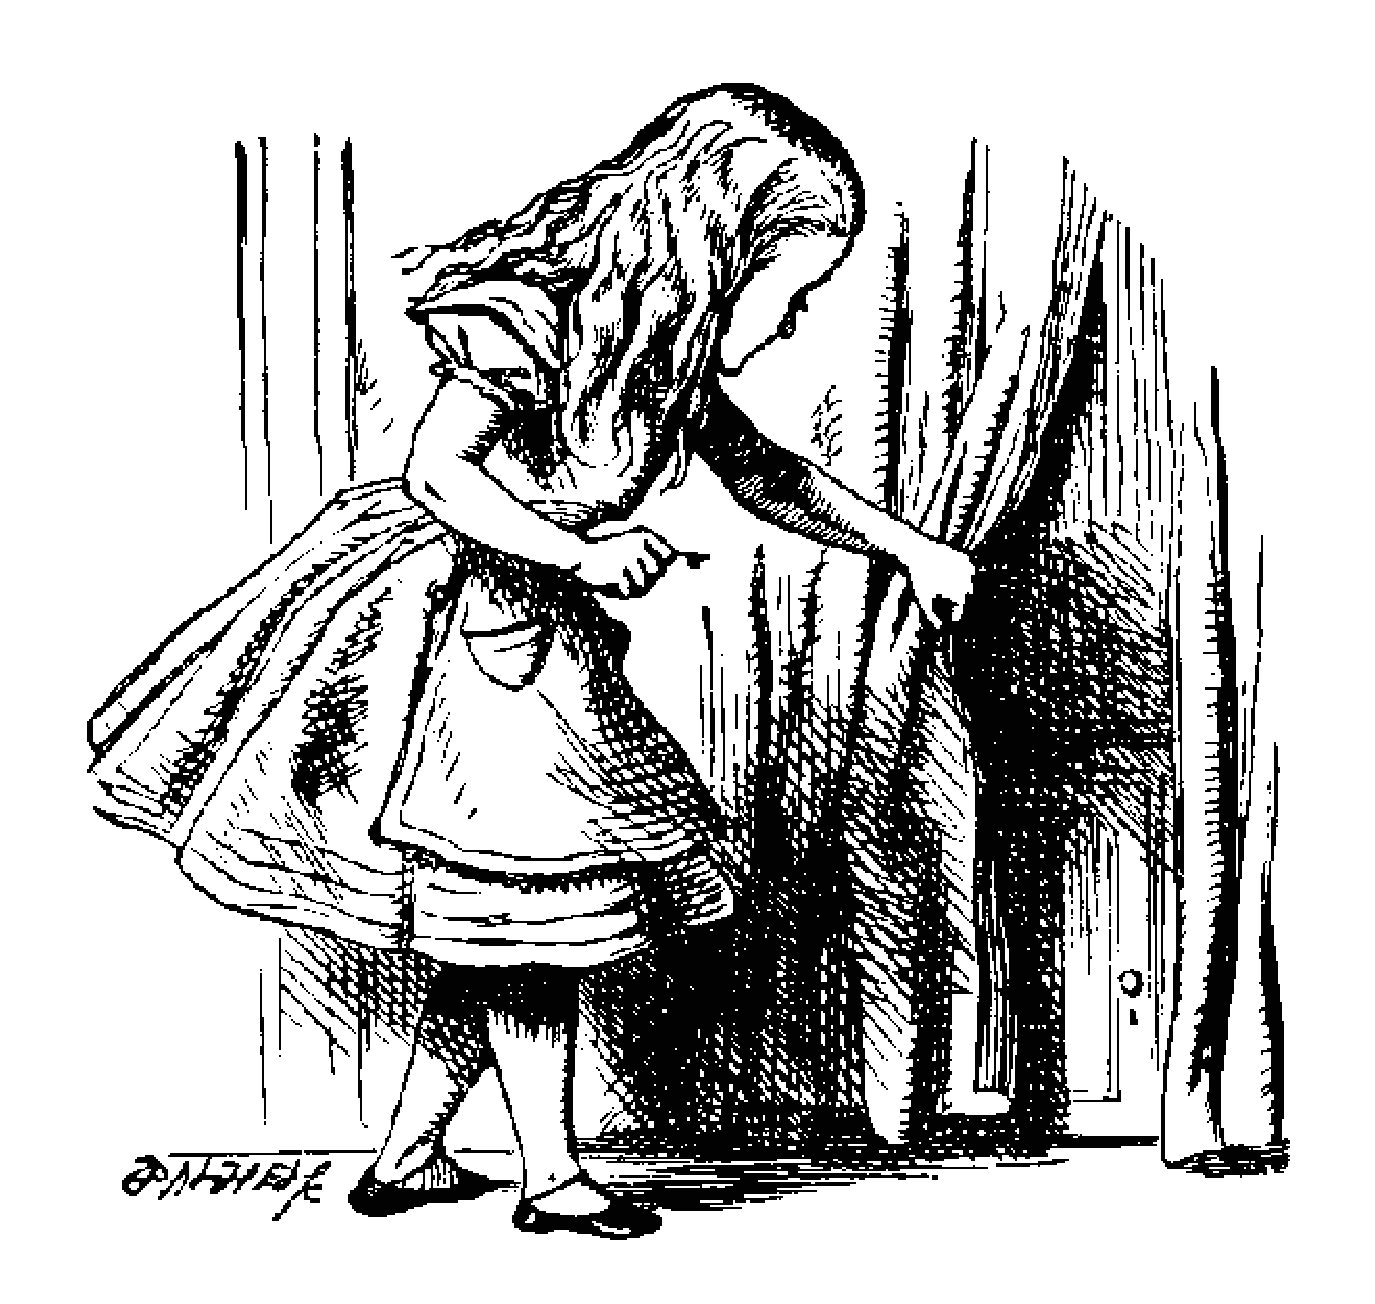
\includegraphics[width=7cm]{figures/alice}
\end{center}
\caption{Behind it was a little door}
\label{fig:alice}
\end{figure}

This is an example of how to reference an inlcuded figure (see Figure \ref{fig:alice}).

%==============================================================================
\section{Reflections}
\label{sec:reflections}
% ##################################################
% LAST EDIT: 	14/03/17	Joseph
% NOTE:	Currently misc. thoughts / notes
% ##################################################

% Several sections that reflect on your experiences during the team project. Each section should discuss one theme, characterised by incidents or events that occurred during the team course of the project from which you learned (approximately 12-15 pages).

\subsection{REFLECTION POINT - Scrum vs XP}
\label{scrumvsxp}
% ##################################################
% LAST EDIT:  15/03/17  Joseph
% NOTE:         Temp notes / thoughts
% ##################################################
This would be a reflection on using the Scrum system in comparison to another system such as Extreme Programming which might have been more suited to our project given its vague nature at the start and would also have helped combat the issues of code reviews / testing.

We ended up with this weird cross system that was mainly Scrum.

Probably pick one then compare against the other and determine if that would have worked better. Probably closer to Scrum of the above two.

Misc points:
\begin{itemize}
\item Time between meetings served as a good sprint dates - working on smaller iterations may have ensured better communication within the team.
\item Development typically did not change much within a sprint - XP difference here may not have made much of a difference though the dropped feature could have been explored earlier in the development cycle than the 2nd semester.
\item Task priority was a bit of an issue as we didn’t really do proper task estimation - XP would have solved that issue as it forces strict policy and task estimation.
\item Scrum has no engineering practices whereas our project definitely should have. XP would have forced pair programming from the start (rather than sporadic occurrences within sprints), ensured better, more thorough testing from an earlier stage in the project and avoided the whole code review “you deleted all my code you bastard” arguments.
\end{itemize}

% ################# Comment Log ####################
% ##################################################


\subsection{REFLECTION POINT - Team Structure}
\label{teamstructure}
% ##################################################
% LAST EDIT:  15/03/17  Joseph
% NOTE:         Temp notes / thoughts
% ##################################################

REFLECTION POINT - Anarchy into Structure (Team Structure)
Initially the team had no real structure and instead utilised a developer anarchy team structure whereby someone would work on whatever system of the felt like at a given time. This eventually stopped working as the team subdivided into divisions - front end, back end and testing with back end being further divided into collaborative filter, evaluator, content based, NEO recommender.

Anarchy would explain the lack of time estimates and product owner however.

Reasons for the failure of the anarchy include the following reasons:

\begin{itemize}
\item Failure to communicate between the team - people weren’t discussing what they were actively working on, tickets didn’t reflect what people were working on, people didn’t yield results in an efficient enough manner.
\item Failure to fully understand domain - anarchy structures require huge expertise of the problem domain which regardless of how smart you are you cannot gain a grasp of in a few weeks. There’s a reason we pay for years worth of experience in a field / industry.
\item Motivation took a hit over Christmas (it was the holidays)
\item Lack of trust between team as we had just met.
\end{itemize}

Changing to a more structured development system did have an effect on productivity (testing improved - we actually had some, front end redesign was rad, more defined roles resulted in better communication within the team)

% ################# Comment Log ####################
% ##################################################

\subsection{REFLECTION POINT - Code Reviews \& Branching}
\label{codereviewbranch}
% ##################################################
% LAST EDIT:  15/03/17  Joseph
% NOTE:         Temp notes / thoughts
% ##################################################
We did not do code reviews and this resulted in some ‘tensions’ during the development of the project. Code reviews from the start of the development would have been beneficial for many reasons (see papers).

Misc Points:
\begin{itemize}
\item The system was designed such that branching was unnecessary for the project. Branching was somewhat discouraged throughout the project in order to reduce merge costs / time. Whether the time saved outweighs the time spent fixing and altering other people’s code remains to be seen.
\item Lack of code reviews meant that the code often had inconsistent styling.
\item Lack of code reviews meant a significant portion of time was spent fixing or altering other people's code to work with parts of the system they did not realise they had broken.
\item Lack of code reviews meant code which was WIP was deleted prior to it being fully implemented into the system - again lack of branching issue somewhat.
\end{itemize}

% ################# Comment Log ####################
% ##################################################

\subsection{REFLECTION POINT - Apache Spark}
\label{sparkreflection}
% ##################################################
% LAST EDIT:  15/03/17  Joseph
% NOTE:         Temp notes / thoughts
% ##################################################
Misc Points:
Team decided the entire team should spend time over Christmas playing around with Apache Spark to ensure common understanding of the system between team members. This may not have been the best use of resource and instead team could have split earlier and the front end developers not bothered playing around with it as they did not end up touching it directly during the development of the project. Common knowledge was gained though but a more typical front end, back end split in focus may have been beneficial and resulted in an improved front end application sooner.

% ################# Comment Log ####################
% ##################################################

%==============================================================================
\section{Conclusions}
\label{sec:conclusions}
% A conclusion that draws general and wider lessons from the case study (approximately 1-2 pages)

Explain the wider lessons that you learned about software engineering,
based on the specific issues discussed in previous sections.  Reflect
on the extent to which these lessons could be generalised to other
types of software project.  Relate the wider lessons to others
reported in case studies in the software engineering literature.

%==============================================================================
\bibliographystyle{plain}
\bibliography{dissertation}
\end{document}
